\documentclass[aps, prb, 11pt, notitlepage]{revtex4-1}
\usepackage{graphicx}
\usepackage{subfigure}
\usepackage{amsmath}
\usepackage[bookmarks, hyperindex, colorlinks=true,
            linkcolor=red,
            urlcolor=blue, citecolor=blue]{hyperref}
   
\usepackage{listings}
\lstset{
  basicstyle=\ttfamily\footnotesize,
  showstringspaces=false,
  commentstyle=\color{Maroon},
  keywordstyle=\color{Blue},
  tabsize=4,
  frame=lines
}

\usepackage{bm}
\usepackage{mwe} 
\usepackage[usenames,dvipsnames,svgnames,table]{xcolor}

%\def\comment#1{\textcolor{red}{#1}}
\renewcommand{\vec}[1]{\bm{#1}}
\renewcommand{\baselinestretch}{1.2}
\def\keywords#1{\textcolor{blue}{{\bf #1}}}
\def\function#1{\textcolor{blue}{{\it #1}}}
\usepackage[final]{changes}
\usepackage{changes}
\usepackage{lipsum}
\graphicspath{{./figures/}}

\makeatletter

\begin{document}
\title{Cache VOL: Efficient Parallel I/O through Caching Data on the Node-local Storage}
\author{Huihuo Zheng$^1$, Venkatram Vishwanath$^1$}
\affiliation{
$^1$Argonne Leadership Computing Facility, 
\\ Argonne National Laboratory, Lemont, IL 60439}
\author{Quincey Koziol$^2$, Houjun Tang$^2$, Suren Byna$^2$, Tonglin Li$^2$}
\affiliation{
$^2$Scientific Data Management Group, \\
Lawrence Berkeley National Laboratory, Berkeley, CA 94720}
\date{\today}
\begin{abstract}
Many high performance computing clusters have two types of storage, a remote storage media of the global parallel file system such as Lustre or GPFS, and node-local storage attached to the compute nodes such as SSDs and NVMe. To our knowledge, the node-local storage are rarely integrated into the parallel I/O workflows in real applications. We present an approach inside the HDF5 library to incorporate node-local storage as a cache to the parallel file system to improve the parallel I/O efficiency. We implemented the feature within the HDF5 Virtual Object Layer framework so that the existing HDF5 applications can use the feature with minimal modification of the codes. This document outline the details of our prototype design as well as initial performance evaluation on Theta at Argonne Leadership Computing Facility, and Summit at Oak Ridge Leadership Computing Facility. 
\end{abstract}
\maketitle
\section{Introduction}
\label{sec:intro}
Many high performance computing (HPC) clusters use a global parallel file system such as Lustre or GPFS for a high I/O throughput. The parallel file system storage are usually separated from the compute nodes. I/O access thus involves transferring data between the global storage media and the compute nodes through the interconnect. Besides the remote storage, the compute nodes are often equipped with node-local storage (NLS) such as SSDs.\cite{theta, summit}
Unfortunately, these NLS are only accessible during the simulation and each of NLS is visible only to those processes on the same compute node. The distributed nature make it not very straight forward to be integrated into the parallel I/O workflows in current existing applications. To our best knowledge, very rare teams have made full usage of these NLS. 

We present here a prototype design of incorporating the NLS into the parallel write and read within the HDF5 library \cite{hdf5}. For parallel write, the main design is to write the data to the NLS first, and then migrate them to the parallel file system asynchronously using background threads. Generally, there is compute work right after the I/O, which can be overlapped with the asynchronous data migration to hide the overall I/O overhead. Outwardly, the I/O performance is determined by bandwidth of synchronous part, i.e., writing data to the NLS. We expect this design will benefit those heavy check-pointing simulations, such as particle based dynamic simulation. ECP applications, such as LAMMPS \cite{lammps}, HACC \cite{hacc} will benefit from this implementation. 

For parallel read, we focus on repeated read workloads, such as deep learning workloads. In such workloads, the same dataset is being read again and again at each iteration, typically in a batch streaming fashion. The workloads are typically distributed in nature with data parallelism. We propose to asynchronously cache the data to the NLS at first iteration so that the application could directly read data from the NLS in later iterations without going to the parallel file system. We expect this will greatly improve the I/O throughput as well as scaling efficiency. Since the caching process is performed using background thread, we expect the same throughput for the first iteration. We expect various deep learning based ECP projects, such as ExaLearn \cite{exalearn}, CANDLE \cite{candle} will benefit from this implementation.

In order to make it easily adopted by the application developers with minimal changes of the codes, we implement everything within the HDF5 Virtual Object Layer (VOL) \cite{vol}. The VOL is an abstraction layer within the HDF5 library that intercepts object-level API operations on HDF5 files (such as ``file open", ``dataset write", ``group create", etc) and can forward those operations to plugins, called ``VOL connectors". These connectors are dynamically loadable at runtime and enable third-party developers to build customized storage solutions for HDF5 users without having to change application code. Therefore, HDF5 applications can benefit from new optimizations and capabilities with ease. Within the VOL framework, we maintain the same API functions such as H5Fcreate/H5Fopen, H5Dwrite/H5Dread and hide all the complexity within the library itself, so that the application developers do not need to deal with the storage hierarchy by themself. However, we also allow the users to specify how to use the NLS through environmental variables. We also provide various API functions for more transparent control of the NLS. 

The organization of this document is as follows. We first outline our design and implementation of the Cache VOL in Section~\ref{sec:design}, and then present some initial performance evaluations on Theta and Summit in Section~\ref{sec:benchmarks}. We briefly discuss our future work in integrating Cache VOL with Async VOL in Section~\ref{sec:future}.
\section{Design and implementation of the Cache VOL} \label{sec:design}
\subsection{Parallel write}
In the parallel write case, we use the NLS to stage the data before writing to the parallel file system. The whole design is schematically shown in Fig.~\ref{fig:schematic}. Instead of directly writing data to the parallel file system, we first write them to the NLS using POSIX write and then migrate them from NLS to the parallel file system in the background asynchronously using native HDF5 dataset write function. The only I/O cost is from the POSIX write since the data migration from the NLS to the filesystem will be hidden under the computation. The POSIX write is local to each rank and does not have any network contention. 

Typically the NLS have a much higher aggregate I/O bandwidth than the parallel file system. For example, on Theta, a XC40 system at ALCF, each node is attached with a SSD with a write rate approximately 500 MB. The aggregate write rate of the full Theta system is 2 TB, whereas the peak bandwidth of the Lustre file system is only about 200 GB. Therefore, by using the NLS to stage the data will effectively improve the parallel I/O throughput at large scale. 
\begin{figure}[hbt]
\centering
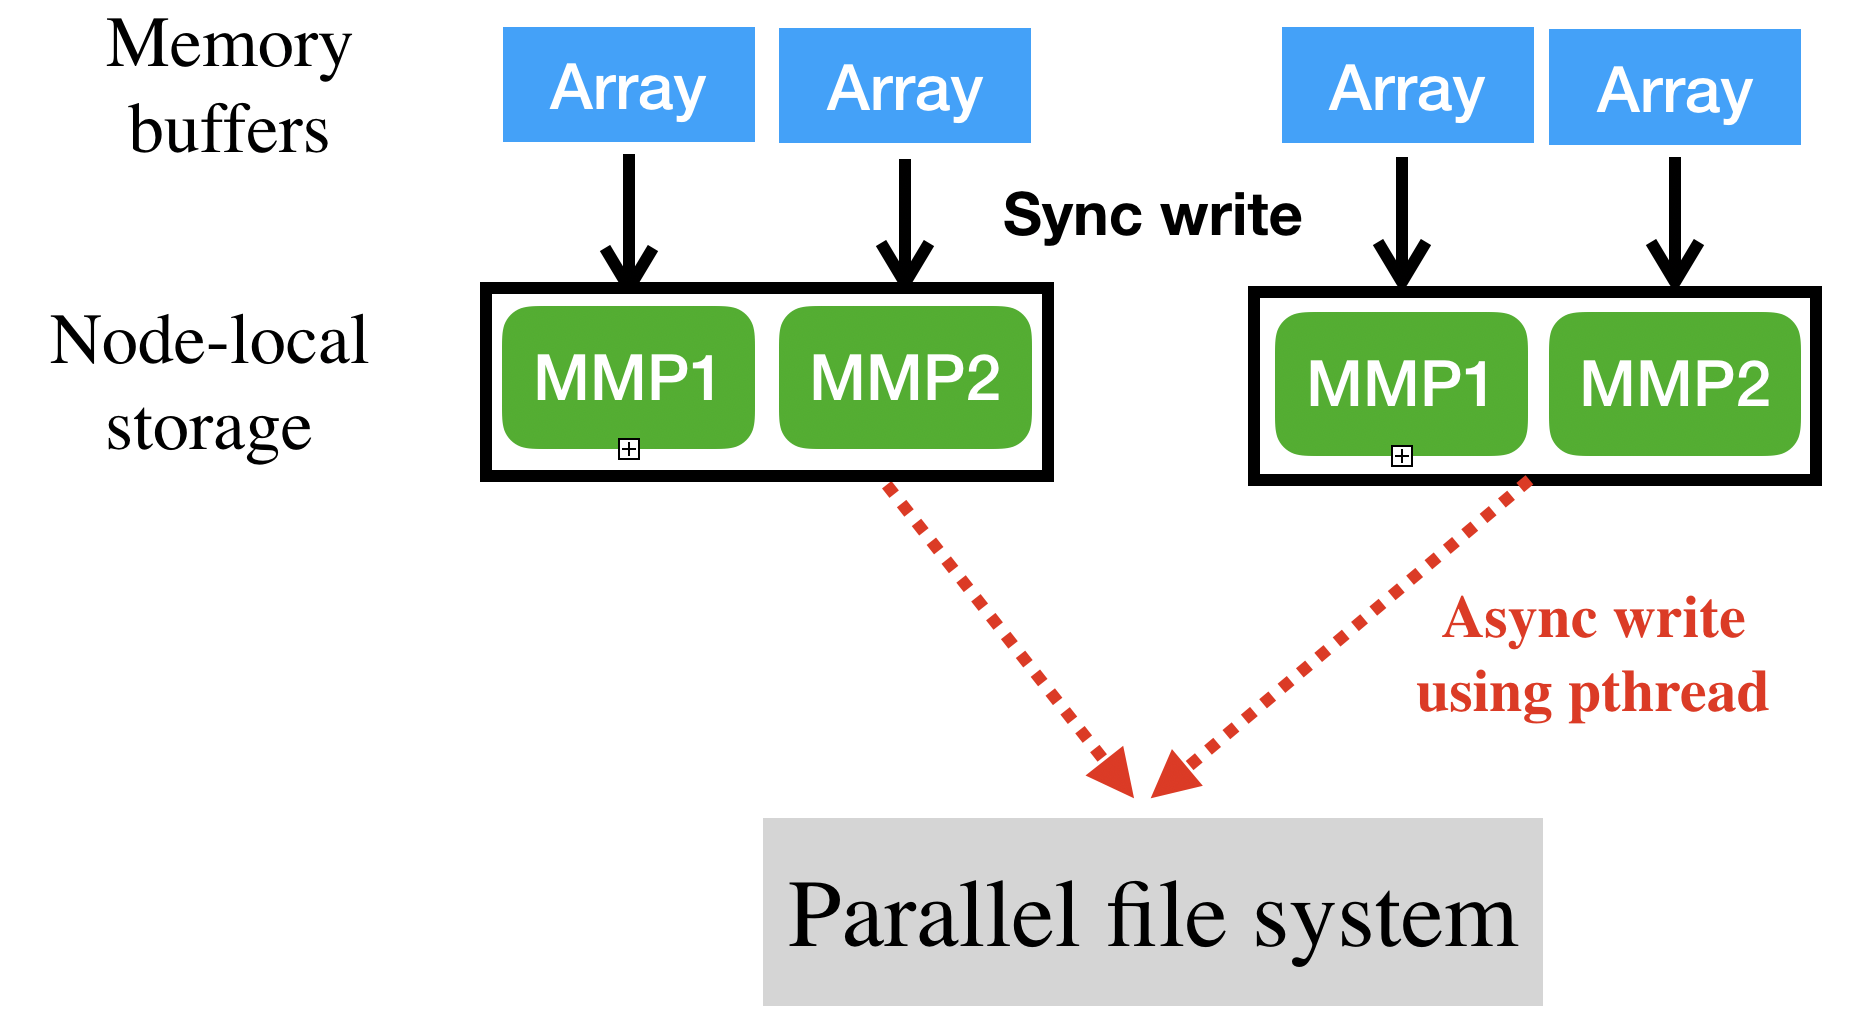
\includegraphics[width=0.8\textwidth]{schematic.png}
\caption{Schematic demonstration of incorporating node-local storage into the parallel I/O workflow. The memory buffers are written into the node-local storage first, and then migrated to the file system asynchronously by a pthread through parallel I/O function calls.}\label{fig:schematic}
\end{figure} 

In order to make the behavior of the dataset write function as similar to the native one as possible, so that the application can adopt the new design without making too much changes in the code, we have the design consideration: 
\begin{itemize}
\item [(1)] The I/O calls shall perform like a blocking I/O calls outwardly. I.e., the buffer should be reusable right after the I/O function returns. We thus make the POSIX write part synchronous, performed through the master thread. We create a pthread to perform the data migration in the background. The I/O function will return right after wakening up the pthread. 
\item [(2)] We shall guarantee all the data being flushed to the file system before closing the dataset or the file. In the dataset / file close function, the master thread needs to wait for the I/O thread to finish the relevant I/O tasks before calling the native dataset / file close function. 
\item [(3)] Ideally, we shall avoid introducing extra memory usage. This can be achieved by using memory mapped file on the NLS. Each rank will create a file on the NLS which will be mapped to a pointer. 
\end{itemize}

With the above consideration, we implement the related callback functions in the Cache VOL: 
\begin{itemize}
\item [(1)] \function{H5VL\_cache\_ext\_file\_create/H5VL\_cache\_ext\_file\_open}: we perform the following three major things for each rank: creating a memory mapped file on the NLS; creating a pthread and putting it into sleep first; calling \function{H5VLfile\_create} / \function{H5VLfile\_open} to create / open a HDF5 file on the file system. 
\item [(2)] \function{H5VL\_cache\_ext\_dataset\_write}: In this function, we write the buffer to the memory mapped file on the NLS, add an I/O task to the task list and waken up the I/O thread. Pthread will then pick a task from the list and execute underlying VOL callback function \function{H5VLdataset\_write} to write the mmap buffer to the file system. We check whether the space left on the NLS is large enough to hold the memory buffer. If not, we put a conditional wait on the master thread to wait until previous I/O tasks have finished. 
\item [(3)]\function{H5VL\_cache\_ext\_file\_close} / \function{H5VL\_cache\_ext\_dataset\_close} : in this function, we put a conditional wait on the master threads to wait for all the relevant I/O tasks to be finished. We then perform \function{H5VLfile\_close} to close the HDF5 file on the file system and remove all the cache files on the NLS. Finally, we join the pthread with the master pthread. 
\end{itemize}

One potential issue of creating pthreads in the library is that it will use extra hardware resource and complete with the application. However, modern HPC platforms become heterogeneous, the majority of the compute works will presumably be offloaded into the accelerators whereas the host might be idle for most of the time. Dedicating one thread on the host to perform I/O shall not degrade the performance of the application too much. 

\subsection{Parallel read}
For parallel read, in order to gain benefit from the NLS, one needs to prefetch the dataset to the NLS and then read from there. However, if the application only reads the data once, it might not have too much benefit to do the prefetch. We thus only consider the repeated read cases such as deep learning applications. In such case, we can cache the dataset to the NLS at first iteration. The future dataset read get data directly from the cache without going again to the file system. 

We assume that the dataset is stored in a one HDF5 file with the following organization: dataset.shape = (nsample, sample.shape), where sample.shape is the shape for each individual sample. {nsample} is the total number of samples in the dataset. During the training, the application sweeps through the entire dataset multiple times, once per epoch. The dataset sometimes is also shuffled in between the two epochs. The whole process is shown in the following pseudo code. 
\begin{lstlisting}[language=c]
for (epoch) { // the application sweep through the entire dataset once per epoch
	for (steps) { // each step, it reads one batch of samples from the dataset. 
		H5_hyperslab_selection(fspace...)  // selection by points 
		...
		H5_hyperslab_selection(fspace...)
		H5Dread( ... fspace, ...buf)
		... // compute work for processing the batch - forward pass + backward pass ... 
	}
}
\end{lstlisting}

Our schematic design for the parallel read workflow is shown in Fig.~\ref{fig:read}. We read the dataset from the file system in the first iteration, and then write it immediately to the local storage asynchronously through pthread.  At future iterations, we will check whether the data is on the NLS or not. If yes, we directly read them there; otherwise, we will go to the file system to get the data. In order to take account of the data shuffling, we create memory buffers the mapped to the files on the NLS. When then the memory buffer to a MPI\_Win so that all the ranks can access remote node NLS in an one-sided communication. 
\begin{figure}[hbt]
\centering
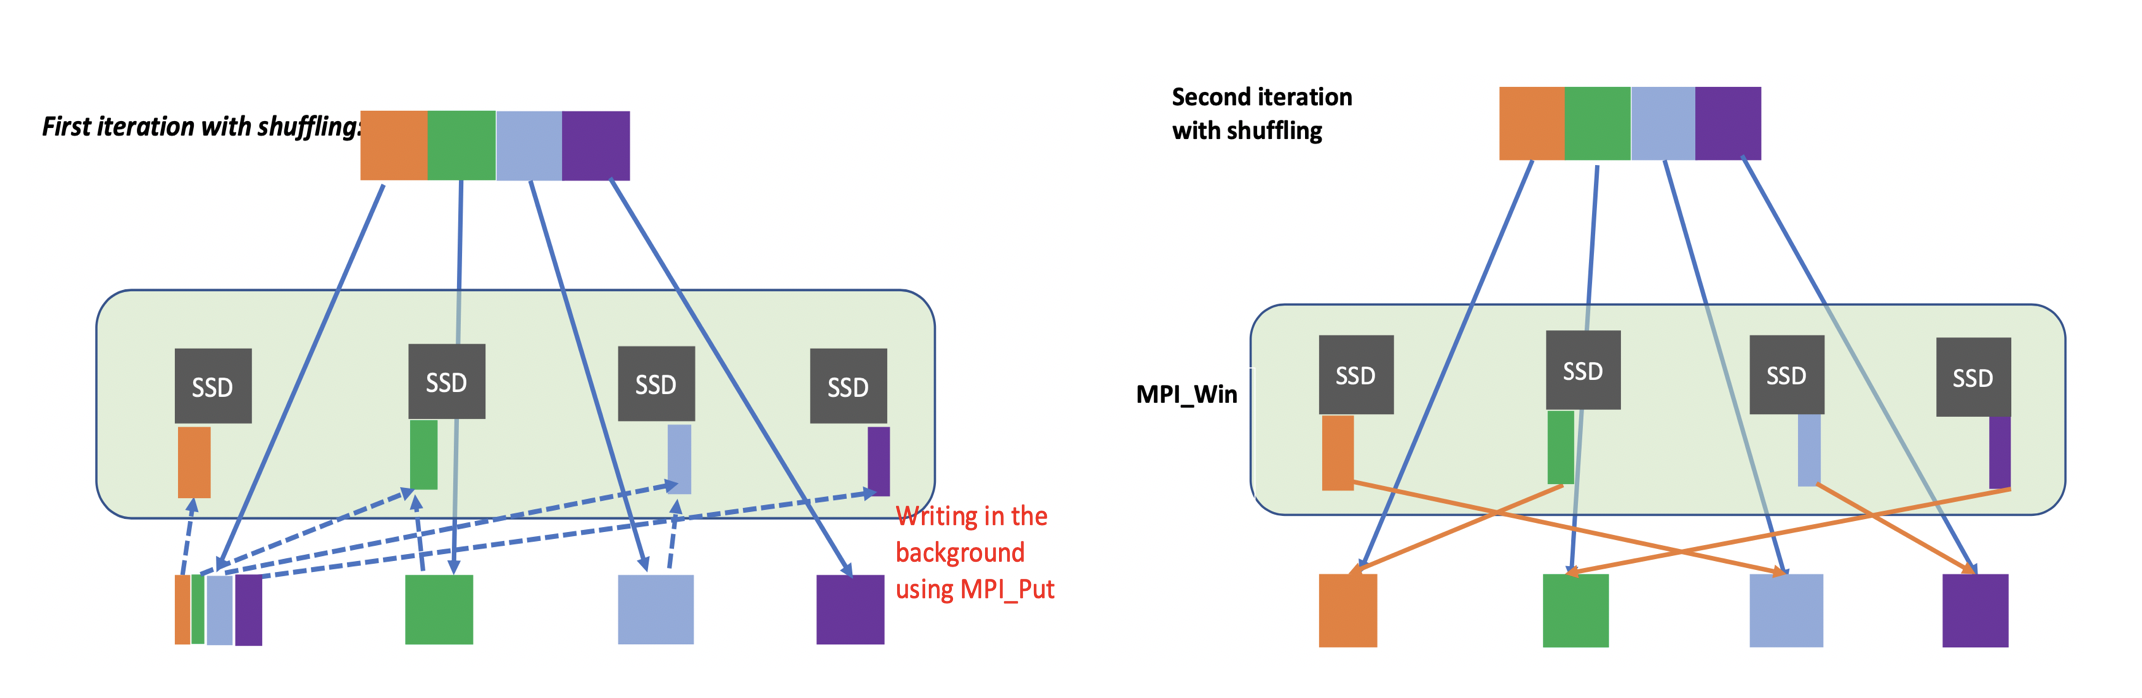
\includegraphics[width=0.9\textwidth]{parallel_read.png}
\caption{Incorporating node-local storage into parallel read workflow. In the first iteration, the data is read from the parallel file system and cached to the node-local storage asynchronously. In the following up iterations, the data is directly fetched from node-local storage without going to the remote file system. Memory map is created for all the cached files on the node-local storage. The memory mapped files are attached to an MPI window. The data caching in the first iteration and data fetching in the following up iterations are performed through one-sided RMA, MPI\_Put and MPI\_Get. If the data can not be fit into the node-local storage entirely, we will have some data left on the file system. In this case, we create another MPI window on the parallel file system, and fetch the rest of the data there. \footnote{Currently, we have not implemented this yet. We assume that the size of the dataset can be fit to the aggregate capacity of all the NLS on the compute nodes.}}\label{fig:read}
\end{figure}

The corresponding VOL callback functions are: 
\begin{itemize}
\item [(1)] \function{H5VL\_cache\_ext\_dataset\_open}: We create memory map files on the node-local storage device. The aggregate size of the memory map files equal to the total size of the dataset. We then create a MPI window and attached the memory mapped buffer to the window. Finally, we then call the underlying VOL function - \function{H5VLdataset\_open} - to open the dataset. 
\item [(2)] \function{H5VL\_cache\_ext\_dataset\_read}: if the dataset to be read has not been cached in the NLS, this function will call \function{H5VLdataset\_read} and then asynchronously store the dataset to the memory map files using pthread with one sided communication - MPI\_Put. If the dataset is already cached in the NLS, this function will call MPI\_Get to directly fetch data from the memory mapped files. 
\item [(3)] \function{H5VL\_cache\_ext\_dataset\_close}: we clear up the memory mapped files on the NLS and then close the dataset by calling \function{H5VLdataset\_close()}. 
\end{itemize}
Notice that \function{H5Dread} function corresponds to \function{H5VL\_cache\_ext\_dataset\_read} which performs prefetching / caching or reading from the NLS cache implicitly. We also implemented the following explicit function: 
\begin{itemize}
\item [(1)] \function{H5Dread\_to\_cache} -- reading data from the parallel file system and write the buffer to the NLS. 
\item [(2)] \function{H5Dread\_from\_cache} -- reading data directly from the NLS.
\end{itemize}

\subsection{Cache management policy and APIs}
When we have multiple files using the NLS while the total capacity of the storage is limited, it is important to manage the resource in an optimal way. In this subsection, we will discuss in details how we managing the caches on the NLS: how to reserve a portion from the storage, how to free up space if storage is full and there are new data to be cached. 

First, we allow each file or dataset to claim a certain portion of space from the NLS for caching its data. A unique folder is created for each HDF5 file to be cached. All the cached data associated to the HDF5 file will be stored inside that folder. In the parallel write implementation, we use the NLS to temporally stage the write buffer and assume that we will not read the data back directly from the NLS.\footnote{We plan to enable RDWR mode in future. In this mode, the application writes the data to the node-local storage, and will be able to read them back to the memory as long as the cache is not cleared.} In such case, we create one memory mapped file per file for each rank. All the buffers associated to the HDF5 file will be stored to this memory mapped file irrespective of which dataset they belong to. All the memory mapped files are located under the same folder mentioned previously. Once the file is closed, we remove the entire folder.  In the parallel read implementation, beside creating a folder for each HDF5 file on the NLS, we also create subfolders for each of the datasets to be cached. All the dataset caches will be placed in the subfolders. The subfolder will be removed once H5Dclose is called, and the top level folder will be removed once H5Fclose is called. 

We define the following properties for the caches: 
\begin{itemize}
\item storage type [SSD/BURST\_BUFFER/MEMORY]. For SSD and BURST\_BUFFER, the path to the storage need to be provided. For MEMORY, RAM will be used to cache the data. 
\item purpose [READ/WRITE/RDWR] - the purpose of this cache, either for read workloads or write workloads, or read and write. Currently, we only focus on the first two modes. RDWR will be supported in future. 
\item duration [PERMANENT/TEMPORAL]: whether the cache is permanent or temporal. 
\begin{itemize}
\item Permanent cache will exist throughout the entire simulation except being explicitly removed. 
\item Temporal cache is removable by the library automatically if another file / dataset is requesting space on the node-local storage while there is not enough space left. By default, all the write cache will be temporary. Once the data is migrated to the parallel file system, the cache is automatically evicted.
\end{itemize}
\item growable [true/false] whether we allow the size to grow or not. 
\item replacement policy [LRU/LFU/FIFO]: the policy to be used for free up space in the node-local storage. 
We take account of each access to the cache, including creation, write / read events. The data eviction for the temporal cache is based on the access info according to the algorithm specified. We currently support LRU, LFU, and FIFO which could be specified through setting \keywords{HDF5\_CACHE\_REPLACEMENT} environmental variable. 
\end{itemize}

Correspondingly, we also define a set of public API functions which allow the application to have fine explicit control of the caches besides the implicit control through environmental variables. 
\begin{itemize} \item Local Storage related functions: 
\begin{itemize}
\item \function {H5Pcreate(H5P\_LOCAL\_STORAGE\_CREATE)} - creating a cache property list
\item \function{H5LScreate(hid\_t plist)} - creating a local storage struct from cache property list.
\item \function{H5LSset()}-- set the information of node-local storage including size, type, path, replacement property
\item \function{H5LSget()} -- query the status of the local storage
\item \function{H5LSclaim\_space(LS, size, char *path, int opt, ...)} -- claim space from the local storage (LS)
\item \function{H5LSregister\_cache (LS, cache)} -- registering a cache to the cache list in the system’s local storage.
\item \function{H5LSremove\_cache(LS, cache)} -- removing a cache and associated files from the system’s local storage.
\item \function{H5LSregister\_access\_count(cache)} -- registering any access events for the cache.
\end{itemize}
\item File cache related functions:
\begin{itemize}
\item \function{H5Pset\_fapl\_cache(plist, flag, value)} - setting the values of cache related variables in the file access property list. Once this is set, cache will be created automatically when H5Fopen or H5Fcreate is called.
\item \function{H5Pget\_fapl\_cache(plist, flag, value)} - setting the values of cache related variables from the file access property list
\item \function{H5Fcache\_create} -- creating a cache in the system’s local storage if it is not yet been created. This is for parallel write. 
\item \function{H5Fcache\_remove} -- removing the cache associated with the file in the system's local storage (This will call \function{H5LSremove\_cache}). After \function{H5Fcache\_remove} is called, \function{H5Dwrite} will directly write data to the parallel file system. 
\end{itemize}
\item Dataset cace related functions (for read only)
\begin{itemize}
\item \function{H5Dcache\_create}-- reserving space for the data
\item \function{H5Dcache\_remove} -- clearing the cache on the local storage related to the dataset Besides these, we will also have the following two functions for prefetching / reading data from the cache
\item \function{H5Dread\_to\_cache} -- pre-fetching the data from the file system and cache them to the local storage
\item \function{H5Dread\_from\_cache} -- reading data from the cache
\end{itemize}
\end{itemize}

By default, the following environmental variables can be specified in the implicit mode. 
\begin{itemize}
\item \keywords{HDF5\_LOCAL\_STORAGE\_PATH} -- path to the local storage, e.g., /local/scratch
\item \keywords{HDF5\_LOCAL\_STORAGE\_SIZE} -- size of the local storage in byte
\item \keywords{HDF5\_LOCAL\_STORAGE\_TYPE} --type of local storage, [SSD/BURST\_BUFFER/MEMORY]
\item \keywords{HDF5\_WRITE\_CACHE\_SIZE} -- the default cache for write [default: 2GB] (noted that we do not have \keywords{HDF5\_READ\_CACHE\_SIZE} because the read cache size will always be the size of the dataset to be cached)
\item \keywords{HDF5\_CACHE\_RD} -- whether to turn on cache for read [yes/no], [default: yes]
\item \keywords{HDF5\_CACHE\_WR} -- whether to turn on cache for write [yes/no], [default: yes]
\item \keywords{HDF5\_CACHE\_REPLACEMENT} -- cache replacement policy: (1) LRU - least recently used [default]; (2) LFU - least frequently used; (3) FIFO - first in first out
\end{itemize}
These environmental variables will have impact on all the file / dataset functions. One can also use H5Pset\_fapl\_cache(plist, flag, value) to achieve the same purpose for a specific file. In such case, flag is name of the environmental variable. 

\subsection{Using local storage cache}
Finally, in real applications, in order to gain benefit from this local-storage implementation,  one should insert enough compute work between \function{H5Dwrite} /  \function{H5Dread} and \function{H5Dclose}. Below are examples of using the Cache VOL.
\begin{itemize}
\item Parallel write \footnote{A complete version of the source code for parallel write: \\https://bitbucket.hdfgroup.org/projects/HDF5VOL/repos/cache/browse/benchmarks/test\_write\_cache.cpp} 
\begin{lstlisting}[language=C++]
#include "H5LS.h"
...
//creating local storage variable through property list
hid_t plist_ls = H5Pcreate(H5P_LOCAL_STORAGE_CREATE); 
LocalStorage *H5LS = H5LScreate(plist_ls);
hid_t plist_id = H5Pcreate(H5P_FILE_ACCESS);
H5Pset_fapl_mpio(plist_id, comm, info);
bool p = true;
// set cache properties in the file access property list, 
// and create the HDF5 with the file access property list.
H5Pset_fapl_cache(plist_id, "LOCAL_STORAGE", H5LS);
H5Pset_fapl_cache(plist_id, "HDF5_CACHE_WR", &p);
H5Fcreate(..., plist_id)
for(int iter=0; iter < nw; nw++)
        H5Dcreate(); 
	... //  other works before I/O
	H5Dwrite(); 
	... // make sure there is compute works to overlap with the data migration
	H5Dclose();
}
H5Fclose()
\end{lstlisting}
\item Parallel read \footnote{A complete version of the source code for parallel read: \\https://bitbucket.hdfgroup.org/projects/HDF5VOL/repos/cache/browse/benchmarks/test\_read\_cache.cpp} 
\begin{lstlisting}[language=C++]
#include "H5LS.h"
//creating local storage variable through property list
hid_t plist_ls = H5Pcreate(H5P_LOCAL_STORAGE_CREATE);
LocalStorage *H5LS = H5LScreate(plist_ls);
hid_t plist_id = H5Pcreate(H5P_FILE_ACCESS);
H5Pset_fapl_mpio(plist_id, comm, info);
bool p = true;
H5Pset_fapl_cache(plist_id, "LOCAL_STORAGE", H5LS);
H5Pset_fapl_cache(plist_id, "HDF5_CACHE_WR", &p);
H5Fopen(..., plist);
H5Dopen();
for(int iw=0; iw < nw; nw++)
	... // some works before I/O
	H5Dread();
	... // compute works to overlap with the data migration
}
H5Dclose();
H5Fclose();
\end{lstlisting}
\end{itemize}

\section{Initial performance evaluation}
\label{sec:benchmarks}
We carried initial performance evaluations for the NLS caching. We put sleep in between H5Dwrite and H5Fclose to mimic computation in the application, we then measure the time spent on H5Dwrite\_cache and calculate the write rate. We perform the evaluation on Theta. The dimension of the local memory space on each rank is $(2048, 2048)$. The dimension of the file space is $(2048\times np\times nw, 2048)$, where $np$ is the number of MPI processes, $nw$ is the number of write. The data is transferred from memory space to the file space through collective MPI I/O. The Lustre stripe setting is stripe count = 48, and stripe size = 16 MB. 


We first test the async feature of the implementation. Without inserting compute in between H5Dwrite and H5Dclose, the data migration time will be manifested in H5Dclose since wait for all the I/O tasks to finish before calling dataset close. As we increase the amount of compute, more and more portion of data migration will overlap with compute, and the time for H5Dclose shall reduce. We perform such a test on 8 nodes, with 32 ranks per node. The local buffer size is set to be 16 MB, and $nw=1$. This is shown in Table~\ref{tab:async}. The time for data migration is about 1.0 second. If the compute is more than 1.0 second, the data migration will be completely hidden. 
\begin{table}[hbt]
\centering
\caption{Time (in second) spent on write and close for different amount of compute. The buffer size is 16 MB. The test is done on 8 KNL nodes, with 32 processes per node. }\label{tab:async}
\begin{tabular}{|l||cccccc|}
\hline
Run & 1 & 2 & 3 & 4 & 5 & 6  \\
\hline
\hline
Compute     & 0.03 &  0.34 & 0.64 & 0.91 & 1.21  & 2.02\\
H5Dwrite &  0.95 & 0.94 & 0.93 &  0.95 & 0.95  & 0.94 \\
H5Dclose & 0.97  & 0.68 & 0.36 & 0.06 & 0.08 & 0.07\\ 
\hline
\hline
Total & 1.95  & 1.96 & 1.93 & 1.92 & 2.24 & 3.03 \\
\hline
\end{tabular}
\end{table}

Next we text the overall ``effective" I/O rate for SSD cache HDF5. We assume that the amount of compute is large enough to overlap with the data migration. Therefore, we measure the time spent on H5Dwrite and compute the I/O bandwidth. We compare it with the I/O bandwidth using H5Dwrite to write directly to the file system. The results are shown in Fig.~\ref{fig:theta_perf} and Fig.~\ref{fig:summit_perf}. 

On Theta, without SSD cache, the collective write rate saturated at about 10 GB/sec. With SSD cache, since the collective write happens in the background, the I/O cost is purely from writing data to SSDs. It scales linearly with respect to the number of nodes as we expected. For the case of 512 nodes, it reaches 250 GB/sec, which is already beyond the peak parallel I/O rate of the Lustre file system. 
\begin{figure}[hbt]
\centering
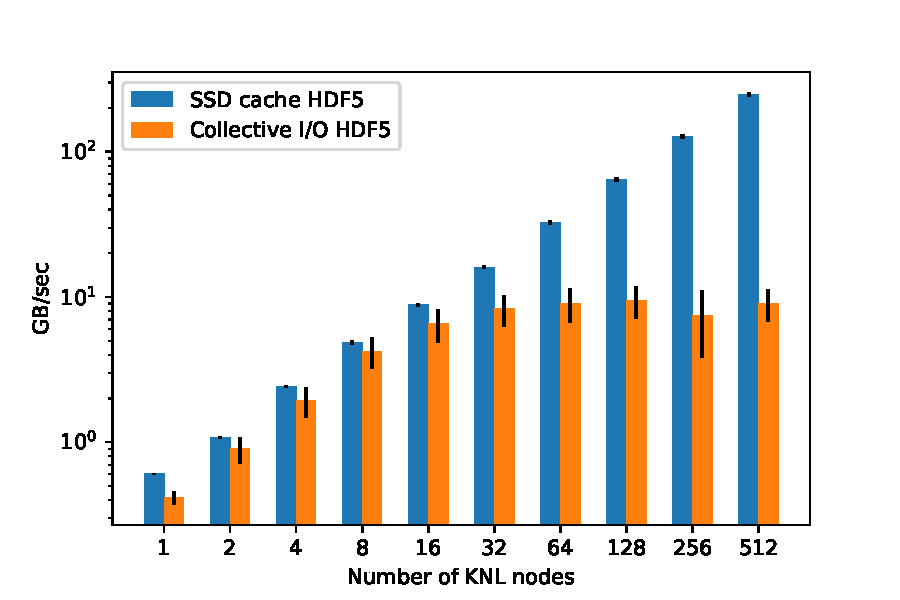
\includegraphics[width=0.6\textwidth]{ssd_cache.pdf}
\caption{HDF5 write rate for collective I/O on Theta Lustre file system. Lustre stripe count is 48, and lustre stripe size is 16MB. The size of the local buffer is 16MB. 32 ranks per node.}\label{fig:theta_perf}
\end{figure}

On Summit, we find the using NVMe as the node-local storage for cache, we are able to achieve about 2GiB/sec/node with almost ideal scaling efficiency. At small scale ($<$256 nodes), directly writing to the GPFS file system has higher bandwidth than using the NLS. This is because per-node I/O bandwidth on GPFS ($\sim 12$GiB/sec) is higher than that on NVMe ($\sim$ 2GiB/sec). However, at large scale ($>$ 256 nodes), directly writing to GPFS has lower bandwidth than writing to NVMe using the Cache VOL. This is because at large scale, the interference from other jobs running on the system becomes severe. At the same time, the scaling bottleneck from the collective I/O in HDF5 start to manifest at large scale. If we use RAM as the NLS for cache, it shows very high bandwidth $\sim 100$ GiB/sec per node. 
\begin{figure}[hbt]
\centering
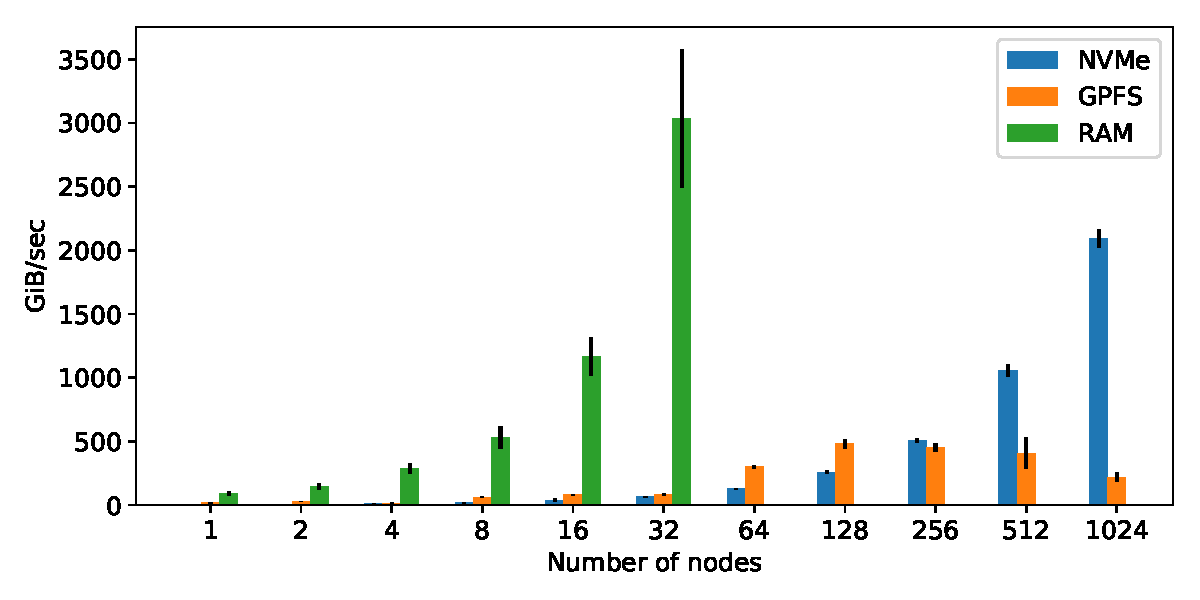
\includegraphics[width=0.8\textwidth]{summit_cache_vol.pdf}\label{sec:summit_perf}
\caption{HDF5 write rate for collective I/O on Summit with (NVMe and RAM) and without (GPFS) the Cache VOL. The size of the write buffer is 16MB on each rank. We set 16 ranks per node.}\label{fig:summit_perf}
\end{figure}
\section{Future work}
\label{sec:future}
Currently, we create a pthread to perform all asynchronous I/O work. One can potentially stack the Async VOL \cite{async_vol} and Cache VOL together and perform the asynchronous I/O work using the Async VOL. 

\section{Conclusion}
We have demonstrated a prototype implementation that incorporating node-local storage into the I/O workflow in the HDF5 Virtual Object Layer framework. In the case of parallel write, we first write the data to local storage and then migrate the data asynchronously to the file system through an I/O helper pthread. Our initial performance evaluation has validated the async I/O feature of this implementation and shown that it can achieve an aggregate effective I/O bandwidth much higher than the peak of the file system. The framework and API are designed in a way that makes the whole framework easy to be adopted by the application developers. 

The source code and the benchmarks code are located at \\https://bitbucket.hdfgroup.org/scm/hdf5vol/cache.git. This TeX source code of this document is included in the ./doc folder in the git repository. 
\section*{Acknowledgment}
This work was supported by the U.S. Department of Energy, Office of Science, Office of Advanced Scientific Computing Research, under contract number DE-AC02-05CH11231 (Project: Exascale Computing Project [ECP] - ExaHDF5 project). This research used resources of the Argonne Leadership Computing Facility, which is a DOE Office of Science User Facility supported under Contract DE-AC02-06CH11357, as well as the Oak Ridge Leadership Computing Facility, which is a DOE Office of Science User Facility supported under Contract DE-AC05-00OR22725.

\bibliographystyle{acm}
\bibliography{cache_vol}
\end{document}
